\documentclass[11pt]{article}
\usepackage{apchem}
\doctitle{Unit 8 Content Guide}
\docsubtitle{A Comprehensive Review of Acids and Bases, Topics 8.1--8.11}
\docstatus{Study draft}
\begin{document}
\titleblock
\begin{abstract}
This guide covers all of Unit 8, Acids and Bases, in twelve sections: one for each of Topics 8.1--8.11 in course order (Topic 8.11, pH and solubility, joined this unit in the Fall 2024 course framework), plus a final section on lab skills and free-response technique. Each section gives the definitions, equations and particle-level reasoning the topic needs, at least one worked example, the phrasing that earns free-response points and the mistakes that cost them. The worked examples use their own acids and numbers, so none of them give away an item in \emph{Unit 8 Practice Set A} or \emph{Unit 8 Practice Set B}. Plan on about 90 minutes for a full read with a calculator out.
\end{abstract}
\leadline{Usage}{first pass, read Sections 1--12 in order and redo every worked example. Then take \emph{Unit 8 Practice Set A} cold; reread the section behind every miss, and take \emph{Unit 8 Practice Set B} two or three days later. The last page is a one-page summary for the night before the unit test. Unit 8 is 11--15\% of the AP multiple-choice section, second only to Unit 3, and a titration question appears in almost every free-response section.}

\section{Introduction to acids and bases (Topic 8.1)}\label{t:8.1}
Water autoionizes: $\ce{2H2O(l) <=> H3O+(aq) + OH-(aq)}$, with
\[ K_w = [\ce{H3O+}][\ce{OH-}] = 1.0\times10^{-14} \text{ at 25 \textdegree C}, \qquad \text{pH} = -\log[\ce{H3O+}], \quad \text{pOH} = -\log[\ce{OH-}], \quad \text{pH} + \text{pOH} = 14.00. \]
\begin{itemize}
\item Neutral means $[\ce{H3O+}] = [\ce{OH-}]$. That is pH 7.00 only at 25 \textdegree C. Autoionization is endothermic, so $K_w$ grows with temperature and neutral pH drops below 7.
\item Brønsted--Lowry acids donate protons; bases accept them. Conjugate pairs differ by one $\ce{H+}$.
\end{itemize}
\worked{1.1} pH 4.30: $[\ce{H3O+}] = 10^{-4.30} = 5.0\times10^{-5}$ M; $[\ce{OH-}] = 2.0\times10^{-10}$ M. Significant figures: the digits after the decimal point in a pH equal the significant figures of the concentration.

\section{pH and pOH of strong acids and bases (Topic 8.2)}\label{t:8.2}
Strong acids (HCl, HBr, HI, $\ce{HNO3}$, $\ce{HClO4}$, $\ce{H2SO4}$) and strong bases (group 1 hydroxides, $\ce{Ca(OH)2}$, $\ce{Sr(OH)2}$, $\ce{Ba(OH)2}$) ionize completely, so concentrations come straight from the formula: 0.015 M $\ce{Sr(OH)2}$ gives $[\ce{OH-}] = 0.030$ M, pOH 1.52, pH 12.48.
\begin{itemize}
\item A tenfold dilution changes pH by one unit (toward 7).
\item Mixing strong acid and strong base: react the moles, then divide the excess by the \emph{total} volume.
\end{itemize}
\worked{2.1} 40.0 mL of 0.150 M HCl + 60.0 mL of 0.120 M KOH: $\ce{H+}$ $6.00\times10^{-3}$, $\ce{OH-}$ $7.20\times10^{-3}$; excess $\ce{OH-}$ $1.20\times10^{-3}$ mol in 0.100 L = 0.0120 M; pOH 1.92; pH 12.08.

\section{Weak acid and base equilibria (Topic 8.3)}\label{t:8.3}
\[ K_a = \frac{[\ce{H3O+}][\ce{A-}]}{[\ce{HA}]}, \qquad K_b = \frac{[\ce{BH+}][\ce{OH-}]}{[\ce{B}]}, \qquad K_aK_b = K_w \text{ for a conjugate pair.} \]
\begin{itemize}
\item pH of a weak acid: $x = [\ce{H3O+}] \approx \sqrt{K_aC}$, valid if $x < 5\%$ of $C$.
\item Percent ionization $= x/C \times 100\%$. It \emph{increases} as the acid is diluted.
\item Conjugate bases of weak acids ($\ce{F-}$, $\ce{CH3COO-}$, $\ce{CN-}$) make basic solutions; conjugate acids of weak bases ($\ce{NH4+}$) make acidic ones. Conjugates of strong acids and bases ($\ce{Cl-}$, $\ce{NO3-}$, $\ce{Na+}$, $\ce{K+}$) are neutral.
\end{itemize}
\worked{3.1} 0.25 M HCN ($K_a = 6.2\times10^{-10}$): $x = \sqrt{1.55\times10^{-10}} = 1.2\times10^{-5}$ M; pH 4.90; 0.0050\% ionized.

\worked{3.2} 0.15 M methylamine ($K_b = 4.4\times10^{-4}$): $x = \sqrt{6.6\times10^{-5}} = 8.1\times10^{-3}$ M (5.4\%, borderline; the exact quadratic gives $7.9\times10^{-3}$); pOH 2.09--2.10, pH 11.9.

\worked{3.3} 0.20 M KF ($K_a$ of HF $6.8\times10^{-4}$): $K_b = 1.5\times10^{-11}$, $[\ce{OH-}] = \sqrt{2.9\times10^{-12}} = 1.7\times10^{-6}$ M, pH 8.23.

\section{Acid--base reactions and buffers (Topic 8.4)}\label{t:8.4}
\begin{center}
\begin{tabular}{p{0.28\linewidth}p{0.32\linewidth}p{0.3\linewidth}}\toprule
Reactants & Net ionic equation & What is left \\ \midrule
Strong acid + strong base & $\ce{H3O+ + OH- -> 2H2O}$ & excess of either; neutral at equivalence \\
Weak acid + strong base & $\ce{HA + OH- -> A- + H2O}$ & buffer before equivalence; $\ce{A-}$ at equivalence \\
Weak base + strong acid & $\ce{B + H3O+ -> BH+ + H2O}$ & buffer before equivalence; $\ce{BH+}$ at equivalence \\ \bottomrule
\end{tabular}
\end{center}
A \emph{buffer} contains significant amounts of a weak acid and its conjugate base. It can be made directly (HA + NaA) or by partly neutralizing a weak acid with a strong base (or a weak base with a strong acid).

\worked{4.1} 0.20 mol HF + 0.10 mol NaOH in 1.0 L: after reaction 0.10 mol HF and 0.10 mol $\ce{F-}$, a buffer with pH = p$K_a$ = 3.17.

\section{Acid--base titrations (Topic 8.5)}\label{t:8.5}
\begin{center}
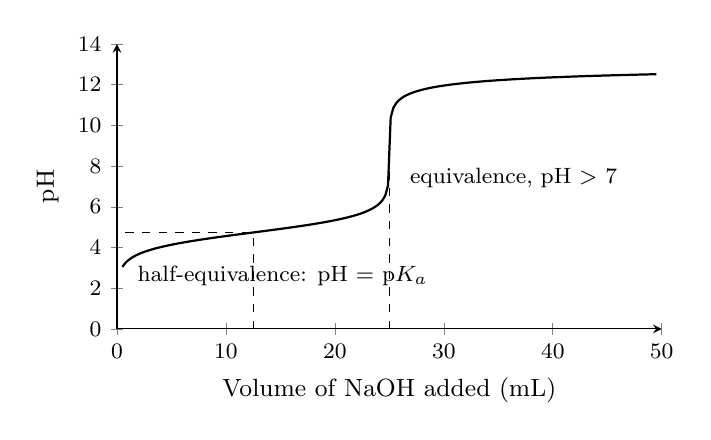
\begin{tikzpicture}
\begin{axis}[width=8.5cm,height=5.2cm,xmin=0,xmax=50,ymin=0,ymax=14,axis lines=left,
  xlabel={Volume of NaOH added (mL)},ylabel={pH},samples=200,domain=0.5:49.5,
  tick label style={font=\footnotesize},label style={font=\small},ytick={0,2,4,6,8,10,12,14}]
\addplot[thick] {x<25 ? 4.74+log10(x/(25-x)) : (x>25 ? 14+log10(0.1*(x-25)/(x+25)) : 8.7)};
\draw[dashed] (axis cs:12.5,0) -- (axis cs:12.5,4.74) -- (axis cs:0,4.74);
\draw[dashed] (axis cs:25,0) -- (axis cs:25,8.7);
\node[font=\footnotesize,anchor=west] at (axis cs:1,2.6) {half-equivalence: pH = p$K_a$};
\node[font=\footnotesize,anchor=west] at (axis cs:26,7.4) {equivalence, pH $>$ 7};
\end{axis}
\end{tikzpicture}

{\small\itshape Weak acid ($K_a = 1.8\times10^{-5}$) titrated with strong base (schematic; the curve near 0 mL is idealized).}
\end{center}
\begin{itemize}
\item \emph{Before any titrant}: pH of the weak acid alone.
\item \emph{Buffer region}: Henderson--Hasselbalch. At \emph{half-equivalence}, [HA] = [$\ce{A-}$] and pH = p$K_a$ (the easiest way to read $K_a$ off a curve).
\item \emph{Equivalence}: only the conjugate base (or acid) remains, so the pH is above 7 for a weak acid and below 7 for a weak base. Strong--strong: pH 7.
\item \emph{After equivalence}: excess strong titrant controls the pH.
\item Polyprotic acids show one equivalence point per proton, at equal volume intervals.
\item Choose an indicator whose color change (p$K_a$ of the indicator $\pm 1$) contains the equivalence pH.
\end{itemize}
\worked{5.1} 30.0 mL of 0.100 M HCOOH (p$K_a$ 3.74) with 0.150 M NaOH: equivalence at 20.0 mL; half-equivalence at 10.0 mL, pH 3.74. At equivalence $[\ce{HCOO-}] = 3.00\times10^{-3}/0.0500 = 0.0600$ M, $K_b = 5.5\times10^{-11}$, $[\ce{OH-}] = 1.8\times10^{-6}$, pH 8.26.

\section{Molecular structure of acids and bases (Topic 8.6)}\label{t:8.6}
An acid is strong when its conjugate base is stable (weakly basic). Structural factors:
\begin{itemize}
\item \emph{Binary acids, same group}: bond strength dominates. HF $\ll$ HCl $<$ HBr $<$ HI (longer, weaker H--X bond).
\item \emph{Binary acids, same period}: bond polarity dominates. $\ce{CH4} < \ce{NH3} < \ce{H2O} < \ce{HF}$.
\item \emph{Oxyacids}: more O atoms, or a more electronegative central atom, pull electron density from the O--H bond and spread the conjugate base's charge. $\ce{HClO} < \ce{HClO2} < \ce{HClO3} < \ce{HClO4}$; $\ce{HOI} < \ce{HOBr} < \ce{HOCl}$.
\item \emph{Carboxylic acids}: the carboxylate ion is resonance-stabilized; electronegative substituents near the carboxyl group strengthen the acid.
\end{itemize}
\worked{6.1} Rank $\ce{H2SO3}$ and $\ce{H2SO4}$: $\ce{H2SO4}$ is stronger (one more O, so its conjugate base spreads the charge over more atoms).

\section{pH and pKa (Topic 8.7)}\label{t:8.7}
\[ \frac{[\ce{A-}]}{[\ce{HA}]} = 10^{(\text{pH} - \text{p}K_a)} \]
\begin{itemize}
\item pH $<$ p$K_a$: protonated form (HA) predominates. pH $>$ p$K_a$: deprotonated form ($\ce{A-}$) predominates. pH = p$K_a$: equal.
\item Indicators: HIn and $\ce{In-}$ have different colors; the color changes over about p$K_a \pm 1$.
\end{itemize}
\worked{7.1} An amino acid side chain with p$K_a$ 10.5 at physiological pH 7.4 is $10^{-3.1}$, about 1/1300, deprotonated: almost entirely the protonated form.

\section{Properties of buffers (Topic 8.8)}\label{t:8.8}
A buffer resists changes in pH because each of its components neutralizes one kind of added strong acid or base:
\[ \text{added acid: } \ce{A- + H3O+ -> HA + H2O} \qquad \text{added base: } \ce{HA + OH- -> A- + H2O} \]
The strong acid or base is replaced by a weak one, so the ratio [A$^-$]/[HA], and so the pH, changes only a little. Choose a conjugate pair with p$K_a$ within about one unit of the target pH.

\section{Henderson--Hasselbalch equation (Topic 8.9)}\label{t:8.9}
\[ \text{pH} = \text{p}K_a + \log\frac{[\ce{A-}]}{[\ce{HA}]} \]
Because both species are in the same volume, you may use moles instead of concentrations. When strong acid or base is added, do the stoichiometry \emph{first} (in moles), then apply the equation.

\worked{9.1} 1.00 L of buffer with 0.300 mol HCOOH and 0.200 mol $\ce{HCOO-}$ (p$K_a$ 3.74): pH = 3.74 + log(0.200/0.300) = 3.56. Add 0.050 mol NaOH: HCOOH 0.250, $\ce{HCOO-}$ 0.250, pH 3.74.

\section{Buffer capacity (Topic 8.10)}\label{t:8.10}
\emph{Buffer capacity} is the amount of strong acid or base a buffer can absorb before its pH changes greatly. It increases with the amounts of HA and $\ce{A-}$ and is greatest when they are equal. A buffer with more $\ce{A-}$ than HA resists added acid better than added base, and the reverse. Diluting a buffer leaves its pH unchanged but lowers its capacity.

\section{pH and solubility (Topic 8.11)}\label{t:8.11}
If a slightly soluble salt contains a basic anion ($\ce{OH-}$, $\ce{F-}$, $\ce{CO3^2-}$, $\ce{PO4^3-}$, $\ce{S^2-}$), lowering the pH removes that anion (by protonating it), so Q falls below $K_{sp}$ and more solid dissolves. Salts of anions from strong acids ($\ce{Cl-}$, $\ce{Br-}$, $\ce{I-}$, $\ce{NO3-}$) are unaffected by pH.

For a hydroxide in a buffered solution, $[\ce{OH-}]$ is fixed by the pH: $s = K_{sp}/[\ce{OH-}]^n$.

\worked{11.1} $\ce{Al(OH)3}$, $K_{sp} = 1.3\times10^{-33}$, at pH 5.00: $[\ce{OH-}] = 1.0\times10^{-9}$, $s = 1.3\times10^{-33}/10^{-27} = 1.3\times10^{-6}$ M. At pH 4.00 it is 1000 times larger.

\section{Lab skills and free-response technique}\label{t:lab}
\begin{itemize}
\item Titration curves: read the equivalence volume at the steepest point; read p$K_a$ at half that volume.
\item Standardize NaOH (it absorbs $\ce{CO2}$) against a primary standard such as KHP.
\item pH meters must be calibrated with buffers; a probe that reads too high shifts every calculated quantity accordingly.
\item Free-response scoring rewards: the correct dominant species at each stage, a stated approximation, and Henderson--Hasselbalch \emph{after} stoichiometry. Particle-level questions often ask which species is in greater concentration; compare pH with p$K_a$.
\end{itemize}

\clearpage
\section*{Summary: Unit 8 on one page}
Use this page the night before. For any row you cannot explain from memory, reread its section and redo its worked example.

\begin{longtable}{@{}p{0.11\linewidth}p{0.40\linewidth}p{0.43\linewidth}@{}}\toprule
\S{} / Topic & Must know & Key equations and tests \\ \midrule
1 / 8.1 & $K_w$; pH, pOH; neutral = equal & pH + pOH = 14.00 (25 \textdegree C) \\[3pt]
2 / 8.2 & Strong acids/bases ionize fully & react, then excess ÷ total $V$ \\[3pt]
3 / 8.3 & $K_a$, $K_b$; \% ionization; salts & $x \approx \sqrt{KC}$; $K_aK_b = K_w$ \\[3pt]
4 / 8.4 & Net ionic for each acid--base pair; making buffers & half-neutralize a weak acid \\[3pt]
5 / 8.5 & Curve regions; indicators; polyprotic & half-eq.\ pH = p$K_a$; eq.\ pH from conjugate \\[3pt]
6 / 8.6 & Bond strength, polarity, O count, resonance & stable conjugate base = strong acid \\[3pt]
7 / 8.7 & Which form predominates & $[\ce{A-}]/[\ce{HA}] = 10^{\text{pH}-\text{p}K_a}$ \\[3pt]
8 / 8.8 & Each component neutralizes one stress & p$K_a \approx$ target pH \\[3pt]
9 / 8.9 & Henderson--Hasselbalch & stoichiometry first, in moles \\[3pt]
10 / 8.10 & Capacity grows with amounts & dilution: same pH, less capacity \\[3pt]
11 / 8.11 & Basic anions dissolve more in acid & $s = K_{sp}/[\ce{OH-}]^n$ at fixed pH \\ \bottomrule
\end{longtable}
\end{document}
